
%% bare_conf_compsoc.tex
%% V1.4b
%% 2015/08/26
%% by Michael Shell
%% See:
%% http://www.michaelshell.org/
%% for current contact information.
%%
%% This is a skeleton file demonstrating the use of IEEEtran.cls
%% (requires IEEEtran.cls version 1.8b or later) with an IEEE Computer
%% Society conference paper.
%%
%% Support sites:
%% http://www.michaelshell.org/tex/ieeetran/
%% http://www.ctan.org/pkg/ieeetran
%% and
%% http://www.ieee.org/

%%*************************************************************************
%% Legal Notice:
%% This code is offered as-is without any warranty either expressed or
%% implied; without even the implied warranty of MERCHANTABILITY or
%% FITNESS FOR A PARTICULAR PURPOSE!
%% User assumes all risk.
%% In no event shall the IEEE or any contributor to this code be liable for
%% any damages or losses, including, but not limited to, incidental,
%% consequential, or any other damages, resulting from the use or misuse
%% of any information contained here.
%%
%% All comments are the opinions of their respective authors and are not
%% necessarily endorsed by the IEEE.
%%
%% This work is distributed under the LaTeX Project Public License (LPPL)
%% ( http://www.latex-project.org/ ) version 1.3, and may be freely used,
%% distributed and modified. A copy of the LPPL, version 1.3, is included
%% in the base LaTeX documentation of all distributions of LaTeX released
%% 2003/12/01 or later.
%% Retain all contribution notices and credits.
%% ** Modified files should be clearly indicated as such, including  **
%% ** renaming them and changing author support contact information. **
%%*************************************************************************


% *** Authors should verify (and, if needed, correct) their LaTeX system  ***
% *** with the testflow diagnostic prior to trusting their LaTeX platform ***
% *** with production work. The IEEE's font choices and paper sizes can   ***
% *** trigger bugs that do not appear when using other class files.       ***                          ***
% The testflow support page is at:
% http://www.michaelshell.org/tex/testflow/



\documentclass[conference,compsoc]{IEEEtran}
\usepackage{latexsym}
\usepackage{graphicx}
\usepackage{color}
\usepackage{geometry}
\usepackage{empheq}
\usepackage{tikz}
\usepackage{pgfplots}
\usetikzlibrary{shapes.geometric,calc}
\pgfplotsset{compat=1.4}
% \addtolength{\oddsidemargin}{-.875in}
% \addtolength{\evensidemargin}{-.875in}
% \addtolength{\textwidth}{1.75in}
% 
% \addtolength{\topmargin}{-.875in}
% \addtolength{\textheight}{1.75in}
\pgfplotsset{compat=newest} % Allows to place the legend below plot
\usepgfplotslibrary{units} % Allows to enter the units nicely
% Some/most Computer Society conferences require the compsoc mode option,
% but others may want the standard conference format.
%
% If IEEEtran.cls has not been installed into the LaTeX system files,
% manually specify the path to it like:
% \documentclass[conference,compsoc]{../sty/IEEEtran}





% Some very useful LaTeX packages include:
% (uncomment the ones you want to load)


% *** MISC UTILITY PACKAGES ***
%
%\usepackage{ifpdf}
% Heiko Oberdiek's ifpdf.sty is very useful if you need conditional
% compilation based on whether the output is pdf or dvi.
% usage:
% \ifpdf
%   % pdf code
% \else
%   % dvi code
% \fi
% The latest version of ifpdf.sty can be obtained from:
% http://www.ctan.org/pkg/ifpdf
% Also, note that IEEEtran.cls V1.7 and later provides a builtin
% \ifCLASSINFOpdf conditional that works the same way.
% When switching from latex to pdflatex and vice-versa, the compiler may
% have to be run twice to clear warning/error messages.






% *** CITATION PACKAGES ***
%
\ifCLASSOPTIONcompsoc
  % IEEE Computer Society needs nocompress option
  % requires cite.sty v4.0 or later (November 2003)
  \usepackage[nocompress]{cite}
\else
  % normal IEEE
  \usepackage{cite}
\fi
% cite.sty was written by Donald Arseneau
% V1.6 and later of IEEEtran pre-defines the format of the cite.sty package
% \cite{} output to follow that of the IEEE. Loading the cite package will
% result in citation numbers being automatically sorted and properly
% "compressed/ranged". e.g., [1], [9], [2], [7], [5], [6] without using
% cite.sty will become [1], [2], [5]--[7], [9] using cite.sty. cite.sty's
% \cite will automatically add leading space, if needed. Use cite.sty's
% noadjust option (cite.sty V3.8 and later) if you want to turn this off
% such as if a citation ever needs to be enclosed in parenthesis.
% cite.sty is already installed on most LaTeX systems. Be sure and use
% version 5.0 (2009-03-20) and later if using hyperref.sty.
% The latest version can be obtained at:
% http://www.ctan.org/pkg/cite
% The documentation is contained in the cite.sty file itself.
%
% Note that some packages require special options to format as the Computer
% Society requires. In particular, Computer Society  papers do not use
% compressed citation ranges as is done in typical IEEE papers
% (e.g., [1]-[4]). Instead, they list every citation separately in order
% (e.g., [1], [2], [3], [4]). To get the latter we need to load the cite
% package with the nocompress option which is supported by cite.sty v4.0
% and later.





% *** GRAPHICS RELATED PACKAGES ***
%
\ifCLASSINFOpdf
  % \usepackage[pdftex]{graphicx}
  % declare the path(s) where your graphic files are
  % \graphicspath{{../pdf/}{../jpeg/}}
  % and their extensions so you won't have to specify these with
  % every instance of \includegraphics
  % \DeclareGraphicsExtensions{.pdf,.jpeg,.png}
\else
  % or other class option (dvipsone, dvipdf, if not using dvips). graphicx
  % will default to the driver specified in the system graphics.cfg if no
  % driver is specified.
  % \usepackage[dvips]{graphicx}
  % declare the path(s) where your graphic files are
  % \graphicspath{{../eps/}}
  % and their extensions so you won't have to specify these with
  % every instance of \includegraphics
  % \DeclareGraphicsExtensions{.eps}
\fi
% graphicx was written by David Carlisle and Sebastian Rahtz. It is
% required if you want graphics, photos, etc. graphicx.sty is already
% installed on most LaTeX systems. The latest version and documentation
% can be obtained at:
% http://www.ctan.org/pkg/graphicx
% Another good source of documentation is "Using Imported Graphics in
% LaTeX2e" by Keith Reckdahl which can be found at:
% http://www.ctan.org/pkg/epslatex
%
% latex, and pdflatex in dvi mode, support graphics in encapsulated
% postscript (.eps) format. pdflatex in pdf mode supports graphics
% in .pdf, .jpeg, .png and .mps (metapost) formats. Users should ensure
% that all non-photo figures use a vector format (.eps, .pdf, .mps) and
% not a bitmapped formats (.jpeg, .png). The IEEE frowns on bitmapped formats
% which can result in "jaggedy"/blurry rendering of lines and letters as
% well as large increases in file sizes.
%
% You can find documentation about the pdfTeX application at:
% http://www.tug.org/applications/pdftex





% *** MATH PACKAGES ***
%
%\usepackage{amsmath}
% A popular package from the American Mathematical Society that provides
% many useful and powerful commands for dealing with mathematics.
%
% Note that the amsmath package sets \interdisplaylinepenalty to 10000
% thus preventing page breaks from occurring within multiline equations. Use:
%\interdisplaylinepenalty=2500
% after loading amsmath to restore such page breaks as IEEEtran.cls normally
% does. amsmath.sty is already installed on most LaTeX systems. The latest
% version and documentation can be obtained at:
% http://www.ctan.org/pkg/amsmath





% *** SPECIALIZED LIST PACKAGES ***
%
%\usepackage{algorithmic}
% algorithmic.sty was written by Peter Williams and Rogerio Brito.
% This package provides an algorithmic environment fo describing algorithms.
% You can use the algorithmic environment in-text or within a figure
% environment to provide for a floating algorithm. Do NOT use the algorithm
% floating environment provided by algorithm.sty (by the same authors) or
% algorithm2e.sty (by Christophe Fiorio) as the IEEE does not use dedicated
% algorithm float types and packages that provide these will not provide
% correct IEEE style captions. The latest version and documentation of
% algorithmic.sty can be obtained at:
% http://www.ctan.org/pkg/algorithms
% Also of interest may be the (relatively newer and more customizable)
% algorithmicx.sty package by Szasz Janos:
% http://www.ctan.org/pkg/algorithmicx




% *** ALIGNMENT PACKAGES ***
%
%\usepackage{array}
% Frank Mittelbach's and David Carlisle's array.sty patches and improves
% the standard LaTeX2e array and tabular environments to provide better
% appearance and additional user controls. As the default LaTeX2e table
% generation code is lacking to the point of almost being broken with
% respect to the quality of the end results, all users are strongly
% advised to use an enhanced (at the very least that provided by array.sty)
% set of table tools. array.sty is already installed on most systems. The
% latest version and documentation can be obtained at:
% http://www.ctan.org/pkg/array


% IEEEtran contains the IEEEeqnarray family of commands that can be used to
% generate multiline equations as well as matrices, tables, etc., of high
% quality.




% *** SUBFIGURE PACKAGES ***
%\ifCLASSOPTIONcompsoc
%  \usepackage[caption=false,font=footnotesize,labelfont=sf,textfont=sf]{subfig}
%\else
%  \usepackage[caption=false,font=footnotesize]{subfig}
%\fi
% subfig.sty, written by Steven Douglas Cochran, is the modern replacement
% for subfigure.sty, the latter of which is no longer maintained and is
% incompatible with some LaTeX packages including fixltx2e. However,
% subfig.sty requires and automatically loads Axel Sommerfeldt's caption.sty
% which will override IEEEtran.cls' handling of captions and this will result
% in non-IEEE style figure/table captions. To prevent this problem, be sure
% and invoke subfig.sty's "caption=false" package option (available since
% subfig.sty version 1.3, 2005/06/28) as this is will preserve IEEEtran.cls
% handling of captions.
% Note that the Computer Society format requires a sans serif font rather
% than the serif font used in traditional IEEE formatting and thus the need
% to invoke different subfig.sty package options depending on whether
% compsoc mode has been enabled.
%
% The latest version and documentation of subfig.sty can be obtained at:
% http://www.ctan.org/pkg/subfig




% *** FLOAT PACKAGES ***
%
%\usepackage{fixltx2e}
% fixltx2e, the successor to the earlier fix2col.sty, was written by
% Frank Mittelbach and David Carlisle. This package corrects a few problems
% in the LaTeX2e kernel, the most notable of which is that in current
% LaTeX2e releases, the ordering of single and double column floats is not
% guaranteed to be preserved. Thus, an unpatched LaTeX2e can allow a
% single column figure to be placed prior to an earlier double column
% figure.
% Be aware that LaTeX2e kernels dated 2015 and later have fixltx2e.sty's
% corrections already built into the system in which case a warning will
% be issued if an attempt is made to load fixltx2e.sty as it is no longer
% needed.
% The latest version and documentation can be found at:
% http://www.ctan.org/pkg/fixltx2e


%\usepackage{stfloats}
% stfloats.sty was written by Sigitas Tolusis. This package gives LaTeX2e
% the ability to do double column floats at the bottom of the page as well
% as the top. (e.g., "\begin{figure*}[!b]" is not normally possible in
% LaTeX2e). It also provides a command:
%\fnbelowfloat
% to enable the placement of footnotes below bottom floats (the standard
% LaTeX2e kernel puts them above bottom floats). This is an invasive package
% which rewrites many portions of the LaTeX2e float routines. It may not work
% with other packages that modify the LaTeX2e float routines. The latest
% version and documentation can be obtained at:
% http://www.ctan.org/pkg/stfloats
% Do not use the stfloats baselinefloat ability as the IEEE does not allow
% \baselineskip to stretch. Authors submitting work to the IEEE should note
% that the IEEE rarely uses double column equations and that authors should try
% to avoid such use. Do not be tempted to use the cuted.sty or midfloat.sty
% packages (also by Sigitas Tolusis) as the IEEE does not format its papers in
% such ways.
% Do not attempt to use stfloats with fixltx2e as they are incompatible.
% Instead, use Morten Hogholm'a dblfloatfix which combines the features
% of both fixltx2e and stfloats:
%
% \usepackage{dblfloatfix}
% The latest version can be found at:
% http://www.ctan.org/pkg/dblfloatfix




% *** PDF, URL AND HYPERLINK PACKAGES ***
%
%\usepackage{url}
% url.sty was written by Donald Arseneau. It provides better support for
% handling and breaking URLs. url.sty is already installed on most LaTeX
% systems. The latest version and documentation can be obtained at:
% http://www.ctan.org/pkg/url
% Basically, \url{my_url_here}.




% *** Do not adjust lengths that control margins, column widths, etc. ***
% *** Do not use packages that alter fonts (such as pslatex).         ***
% There should be no need to do such things with IEEEtran.cls V1.6 and later.
% (Unless specifically asked to do so by the journal or conference you plan
% to submit to, of course. )


% correct bad hyphenation here
\hyphenation{op-tical net-works semi-conduc-tor}
\geometry{left=2.03cm,right=2.03cm,top=2.95cm,bottom=2.03cm}

\begin{document}
%
% paper title
% Titles are generally capitalized except for words such as a, an, and, as,
% at, but, by, for, in, nor, of, on, or, the, to and up, which are usually
% not capitalized unless they are the first or last word of the title.
% Linebreaks \\ can be used within to get better formatting as desired.
% Do not put math or special symbols in the title.
\title{ESTIMATION OF THERMAL CONTACT CONDUCTANCES ON IRREGULAR
	INTERFACES USING THE GENERALIZED INTEGRAL TRANSFORM
	TECHNIQUE AND THE RECIPROCITY FUNCTIONAL METHOD}




% author names and affiliations
% use a multiple column layout for up to three different
% affiliations
\author{
\IEEEauthorblockN\textbf{Guilherme Camelo de Freitas}
\IEEEauthorblockA{Department of Mechanical Engineering,\\POLI/COPPE\\
Federal University of Rio de Janeiro\\
Rio de Janeiro, RJ, Brazil\\
helcio@mecanica.ufrj.br}
\and
\IEEEauthorblockN\textbf{Marcelo J. Cola\`co}
\IEEEauthorblockA{Department of Mechanical Engineering,\\POLI/COPPE\\
Federal University of Rio de Janeiro, UFRJ\\
Rio de Janeiro, RJ, Brazil\\
colaco@ufrj.br}}

% conference papers do not typically use \thanks and this command
% is locked out in conference mode. If really needed, such as for
% the acknowledgment of grants, issue a \IEEEoverridecommandlockouts
% after \documentclass

% for over three affiliations, or if they all won't fit within the width
% of the page (and note that there is less available width in this regard for
% compsoc conferences compared to traditional conferences), use this
% alternative format:
%
%\author{\IEEEauthorblockN{Michael Shell\IEEEauthorrefmark{1},
%Homer Simpson\IEEEauthorrefmark{2},
%James Kirk\IEEEauthorrefmark{3},
%Montgomery Scott\IEEEauthorrefmark{3} and
%Eldon Tyrell\IEEEauthorrefmark{4}}
%\IEEEauthorblockA{\IEEEauthorrefmark{1}School of Electrical and Computer Engineering\\
%Georgia Institute of Technology,
%Atlanta, Georgia 30332--0250\\ Email: see http://www.michaelshell.org/contact.html}
%\IEEEauthorblockA{\IEEEauthorrefmark{2}Twentieth Century Fox, Springfield, USA\\
%Email: homer@thesimpsons.com}
%\IEEEauthorblockA{\IEEEauthorrefmark{3}Starfleet Academy, San Francisco, California 96678-2391\\
%Telephone: (800) 555--1212, Fax: (888) 555--1212}
%\IEEEauthorblockA{\IEEEauthorrefmark{4}Tyrell Inc., 123 Replicant Street, Los Angeles, California 90210--4321}}




% use for special paper notices
%\IEEEspecialpapernotice{(Invited Paper)}




% make the title area
\maketitle

% As a general rule, do not put math, special symbols or citations
% in the abstract
\begin{abstract}
You can find below the instructions for the preparation of papers for the INVERSE PROBLEMS, DESIGN AND OPTIMIZATION SYMPOSIUM. The length of the paper is limited to \textbf{8 (eight) pages}. The paper must be submitted electronically, in PDF (Portable Document Format) format, as an attachment to an e-mail message to the address:  \textcolor{blue}{\underline {ipdo2019@hebut.edu.cn}}. Please name the file containing your paper according to the number of your abstract/paper, which was sent previously. The name of your file should be as follows: IPDO-.pdf, where  is the number of your paper. You should use the number of your paper as the subject of this e-mail message.

\end{abstract}

% no keywords




% For peer review papers, you can put extra information on the cover
% page as needed:
% \ifCLASSOPTIONpeerreview
% \begin{center} \bfseries EDICS Category: 3-BBND \end{center}
% \fi
%
% For peerreview papers, this IEEEtran command inserts a page break and
% creates the second title. It will be ignored for other modes.

\IEEEpeerreviewmaketitle


\section{Introduction}

If heat transfer takes place through a common boundary between two bodies in physical contact, a discontinuity in the temperature profile is observed across the interface defined by that boundary, which indicates that the thermal contact is not perfect there. The ratio of the heat flux per area unit to the temperature drop, both measured at that interface, is called \textit{thermal contact conductance} (abbreviated as TCC):

\begin{equation}
h_c = \frac{q_c}{\Delta T} \label{definicao_1}
\end{equation}

An equivalent definition of the TCC may be established upon the analysis of the associated heat conduction problem, by means of the boundary conditions evaluated on the contact interface. Thus, if $T_1$ and $T_2$ are the temperature fields in each of the solids whose contact interface is designated by $\Gamma$, and  $k_1$ and $k_2$ are their respective thermal conductivities, then energy balance allows the following relation:

\begin{equation}
-k_1\frac{\partial T_1}{\partial \mathbf{n}_1}\bigg|_\Gamma
=
h_c(T_1 - T_2)_\Gamma
=
k_2\frac{\partial T_2}{\partial \mathbf{n}_2}\bigg|_\Gamma \label{definicao_2}
\end{equation}

which leads to

\begin{equation}
h_c = \frac{-k_1\displaystyle\frac{\partial T_1}{\partial \mathbf{n}_1}\bigg|_\Gamma}{(T_1 - T_2)_\Gamma} = \frac{k_2\displaystyle\frac{\partial T_2}{\partial \mathbf{n}_2}\bigg|_\Gamma}{(T_1 - T_2)_\Gamma} \label{eq:definicao_3}
\end{equation}

The TCC may be seen as a parameter to evaluate the quality of the contact between two solid bodies. In extreme cases, the TCC vanishes on perfect thermally isolated regions along the contact interface, since the heat flux on the numerator in \eqref{definicao_1} will be zero, whereas an infinite value for TCC will be found where the contact itself is perfect, for which the temperature jump on the denominator in \eqref{definicao_1} will be zero. The TCC may also be useful for evaluating the presence of discontinuities or cracks inside heterogeneous materials; in fact, there will be temperature jumps at those regions and the temperature fields measured on the external boundaries of the material will show values different from the expected ones if those discontinuities did not exist. Some examples of the necessity of calculating or estimating the TCC may be found in aerodynamics (citar LAMBERT), microelectronics (citar SNAITH) or heat exchanger projects (citar HUANG). 

Some measuring methods developed for estimating the TCC usually demand knowlegde of details of the surfaces in contact, as well as evaluations of temperature and heat flux inside the bodies in contact, either \textit{in loco} or through some kind of regression from measurements at inner points, resulting in complex or intrusive experimental assemblies (citar bibliografia). Still, due to its special features, this problem may be classified as an Inverse Heat Conduction Problem (abbreviated as IHCP); in that case, the distribution of TCC across the contact interface may be considered as the unknown function to be estimated, by means of the definition \eqref{definicao_1}. In any case, the distributions of heat flux and temperature jumps across the contact interface, which are necessary for estimation of TCC from \eqref{definicao_1}, still need to be measured or calculated.

The concept of Reciprocity Functional (abbreviated as FR), introduced by Andrieux and Ben Abda (citar os trabalhos), has been applied in recent researches on indirect evaluation of temperature jumps and heat flux distributions across contact interfaces (citar os trabalhos de CTC envolvendo FR). These works resulted in development of non-intrusive, non-iterative, and more computationally efficient approaches for estimation of the TCC. However, these techniques have been applied to regular geometrical configurations, such as retangular or circular-shaped cross section contact interfaces. Nevertheless, the analytical development envolving the use of the FR approach is not restricted to any particular geometry, and may be expanded to more compreehensive configurations.

This paper presents and discusses the problem of estimating the TCC between two solid bodies in contact, considering that the contact interface is not necessarily regular. The starting point is the work developed by Alves (citar) and Abreu (citar), who studied the specific case in which the contact interface is plane and horizontal, given that both bodies have a rectangular cross section shape. The auxiliary problems, which provide the necessary functions to be used in the FR approach, were solved using the Method of Fundamantal Solutions. Padilha (citar), by means of the Classic Integral Transform Technique (abbreviated CITT) (citar COTTA), deduced an analytic expression to estimate the TCC for this particular case model. In this work, the contact interface has been represented by an equation $ y = w(x)$, 

\begin{figure}[h!b]
	\begin{center}
		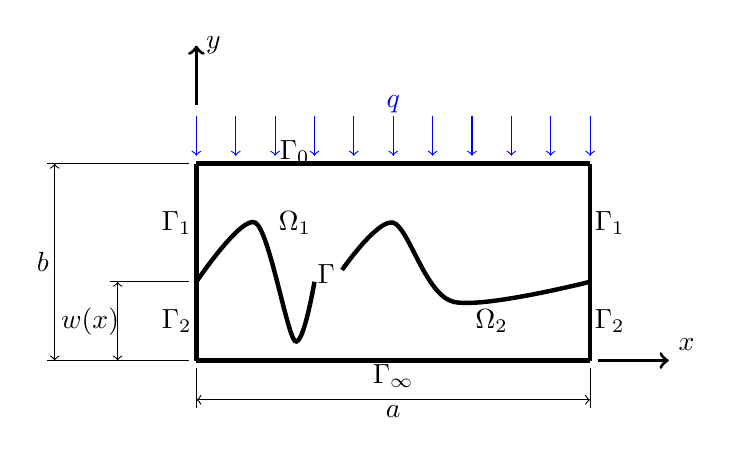
\begin{tikzpicture}[scale=0.5]
		
		\draw [ultra thick] (0, 0) -- (10, 0);
		%\draw [ultra thick] (0, 2) -- (7, 2);
		%\draw [ultra thick] (8, 2) -- (10, 2);
		\draw [ultra thick] plot [smooth] coordinates {(0, 2) (1.5, 3.5) (2.5, 0.5) (3, 2)};
		\draw [ultra thick] plot [smooth] coordinates {(3.7, 2.3) (5, 3.5) (6.5, 1.5) (10, 2)};
		\draw [ultra thick] (0, 5) -- (10, 5);
		\draw [ultra thick] (0, 0) -- (0, 5);
		\draw [ultra thick] (10, 0) -- (10, 5);
		
		\draw (2.5, 3.5) node {$\Omega_1$};
		\draw (7.5, 1) node {$\Omega_2$};	
		\draw (3.3, 2.2) node {$\Gamma$};
		\draw (-0.5, 3.5) node {$\Gamma_1$};
		\draw (-0.5, 1) node {$\Gamma_2$};
		\draw (10.5, 3.5) node {$\Gamma_1$};
		\draw (10.5, 1) node {$\Gamma_2$};
		\draw (5, -0.4) node {$\Gamma_\infty$};
		\draw (2.5, 5.3) node {$\Gamma_0$};
		\draw [blue](5, 6.5) node {$q$};
		\draw (5, -1.3) node {$a$};
		\draw (-3.9, 2.5) node {$b$};
		\draw (-2.7, 1) node {$w(x)$};
		
		\node [above right] at (12, 0) {$x$};
		\node [right] at (0, 8) {$y$};
		
		\draw [->, blue] (0, 6.2) -- (0, 5.2);
		\draw [->, blue] (1, 6.2) -- (1, 5.2);
		\draw [->, blue] (2, 6.2) -- (2, 5.2);
		\draw [->, blue] (3, 6.2) -- (3, 5.2);
		\draw [->, blue] (4, 6.2) -- (4, 5.2);
		\draw [->, blue] (5, 6.2) -- (5, 5.2);
		\draw [->, blue] (6, 6.2) -- (6, 5.2);
		\draw [->, blue] (7, 6.2) -- (7, 5.2);
		\draw [->, blue] (8, 6.2) -- (8, 5.2);
		\draw [->, blue] (9, 6.2) -- (9, 5.2);
		\draw [->, blue] (10, 6.2) -- (10, 5.2);
		
		\draw [->, very thick] (10.2,0) -- (12,0);
		\draw [->, very thick] (0, 6.5) -- (0,8);
		
		\draw [-] (0, -0.2) -- (0, -1.2);
		\draw [-] (10, -0.2) -- (10, -1.2);
		\draw [<->] (0, -1) -- (10, -1);
		
		\draw [-] (-0.2, 0) -- (-3.8, 0);
		\draw [-] (-0.2, 5) -- (-3.8, 5);
		\draw [-] (-0.2, 2) -- (-2.2, 2);
		\draw [<->] (-3.6, 0) -- (-3.6, 5);
		\draw [<->] (-2.0, 0) -- (-2.0, 2);
		
		\end{tikzpicture}
		\caption{Geometria do problema físico}
		\label{fig2}
	\end{center}
\end{figure}



\newpage

The text of your paper must be typed with single spacing, justified, in a 10-point size font and in two columns, except for the title of the paper, authors and affiliations, which appear in a single column on the first page.\\

In your word processor, you should set the size of the paper to 19 cm (7.48 inch) of width and 27 cm (10.63 inch) of height. This size will be printable on both A4 and letter sizes of paper. Set the margins and column widths as specified in Table 1.



\section{TITLE, AUTHORS AND AFFILIATIONS}
The title of your paper should be typed in a single column, in Arial, 12-point size, capital letters and boldface. The title should be centered and beginning on the first line below the top margin.

Leave one blank line (12-point size) below the title and then type names of the authors of the paper in Arial, upper and lower case letters, 10-point size and boldface. On the line exactly below the authors, type the affiliations in Times Roman, italic, upper and lower case letters, 10-point size. You may use more than one line for the affiliation, which should include: (i) Department or division name; (ii) Company or University name; (iii) City and state; (iv) Country; and (v) e-mail address. In the case of a second author with an affiliation different from the first one, place the second author/affiliation beside the first one, as indicated above. If there are more authors with different affiliations, please place them evenly below the first two ones, by leaving one blank line (10-point size) of space between them.

Leave two blank lines (10-point size) below the affiliations and then begin typing the text of your paper in a two-column format. Use the margins, column width and spacing specified in Table 1.\\
\begin{table}[ht]\centering
\caption{Margins and column width}
\begin{tabular}{|l|p{50pt}|p{51pt}|}
\hline
\textbf{Settings} & \multicolumn{2}{|p{102pt}|}{\textbf{Size}}\\ \cline{2-3}
  &\textbf{cm}&\textbf{inch}\\
\hline
Top Margin&2.95&1.16\\
\hline
Bottom Margin&2.03&0.8\\
\hline
Left Margin&2.03&0.8\\
\hline
Right Margin&2.03&0.8\\
\hline
\end{tabular}
\end{table}


\textbf{TEXT}

Your text should begin with an Abstract giving a clear indication of the objectives, scope and main results of the paper. The Abstract should not contain more than 150 words.

Following the Abstract, your paper should contain the Nomenclature, with the list and definitions of the most important symbols used. The Nomenclature list should be in alphabetical order, followed by Greek symbols, subscripts and superscripts, identified with pertinent headings.

The text of your paper should be typed in Times Roman, 10-point size, justified and with single spacing. Paragraphs should be indented 0.5 cm (0.20 in).

The following text should appear as a header on all pages:

1$^{st}$ line:\textit{ Inverse Problems, Design and Optimization Symposium -- IPDO2019}

2$^{nd}$ line: \textit{Tianjin, China, September 24-26, 2019}

The header should be typed flush left with the left margin in Times Roman, 10-point size and in italic. The header should be placed at 1.25 cm (0.49 in) from the top of the page. Please avoid the use of footnotes.

Primary text headings should be in Arial, 10-point size, boldface, in capital letters and flush left with the left margin. If the heading runs for more than one line, the run-over text should also be flush left with the left margin. There should be one line space above primary headings. Text begins on the line following the heading.


\textbf{FIGURES}

Figures must be embedded in your text and appear as close as possible to its first reference. All figures (graphs, line drawings, photographs, etc.) should be numbered consecutively and have a caption consisting of the figure number and a brief title. This number should be used when referring to the figure in the text. All figures should be referenced in the text. The caption should be placed under the figure and both figure and caption should be centered. There should be a minimum of one empty line above the figure and between figure caption and the text (see Fig. 1 as an example).
\begin{center}
%%\begin{figure}[htbp]
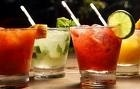
\includegraphics[width=130pt, height=82pt, keepaspectratio=true]{f1.jpg}
%%\caption{This should be the caption for \texttt{f1.jpg}.}
%%\end{figure}

Fig. 1. Scheme of the drying experiment
\end{center}


\textbf{TABLES}

All tables should be numbered consecutively and have a caption consisting of the table number and a brief title. This number should be used when referring to the table in the text. Tables should be inserted as part of the text, as close as possible to their first reference. All tables should be referenced in the text. The caption should be placed above the table and both table and caption should be centered. There should be one empty line between the text and the table title and between table and the text (see Table 1 as an example).

All tables should be numbered consecutively and have a caption consisting of the table number and a brief title. This number should be used when referring to the table in the text. Tables should be inserted as part of the text, as close as possible to its first reference. All tables should be referenced in the text. The caption should be placed above the table and both table and caption should be centered. There should be a minimum of one empty line above the table caption and between the table and text (see Table 1 as an example).


\textbf{EQUATIONS}

All equations should start from the left margin of a column and be numbered consecutively beginning with (1). The equation number should be enclosed in parentheses and set flush right in the column. It is this number that should be used when referring to equations within the text.

\begin{equation}
\label{eq1}
E=m\varsigma^{2}
\end{equation}

Formulas and equations should be created to clearly distinguish capital letters from lowercase letters. Care should be taken to avoid confusion between the lowercase "l'' (el) and the numeral one,or between zero and the lowercase "o.'' All subscripts, superscripts, Greek letters, and other symbols should be clearly indicated.

In all mathematical expressions and analyses, any symbols not previously defined in the Nomenclature should be explained.

There should be one empty line between equations and text and between the consecutive equations.

SI units must be used.


\textbf{REFERENCES}

References are indicated in the text by consecutive Arabic numbers in square
brackets such as [2], numbered in accordance with the order of appearance.
The references should be collected at the end of the text in numerical order
and should follow the form suggested in the journal \textit{Inverse Problems in Science and Engineering,} in the corresponding
file to be downloaded in the section ``Style guidelines''\\
\textcolor{blue}{\underline{(http://www.tandfonline.com/action/authorSubmi}}
\textcolor{blue}{\underline{ssion?journalCode=gipe20\&page=instructions)}}.

Some examples are:

\noindent 1. A. Brown, Diamond-anvil studies at high pressure, \textit{Phys. Rev., B}, \textbf{26}, 5668
(1992).

\noindent 2. J. P. Hansen and I. R. McDonald, \textit{Theory of Simple Liquids}, Academic Press, New York, p. 426,
(1976).

\hangafter 1
\hangindent 1em
\noindent 3. K. Fukutani and A. Shakouri, Optimization of thin film iicrocoolers for
hot spot removal in packaged integrated circuit chips, \textit{22nd IEEE SEMI-THERM Symposium}, Dallas, Texas, pp.
\noindent 130-134, March 14-16 (2006).

\noindent 4. V. Rieke and k. Butts Pauly, MR thermometry, \textit{J. of Magnetic Resonan. Imag.}, \textbf{27}(2), 376--390
(2008).





\end{document}


